% IEEE Technical Report style draft for ZTA project
% Compile: pdflatex final_report.tex
\documentclass[conference]{IEEEtran}

\usepackage{graphicx}
\usepackage{booktabs}
\usepackage{tabularx}
\usepackage{url}
\usepackage{float}
\usepackage{tikz}
\usetikzlibrary{positioning,arrows.meta}

\title{Zero Trust Architecture Sandbox: Implementation and Evaluation Report}

\author{Minsoo Ahn\\
Student ID: 114743792\\
CSE 487 T92\\
Instructor: Antonino Mione\\
Date: May 11, 2026}

\begin{document}
\maketitle

\begin{abstract}
This report describes a hands-on implementation of a Zero Trust Architecture (ZTA)
using an open-source stack on a local Kubernetes cluster. The system follows NIST SP
800-207 principles with Istio as the policy enforcement point, OPA as the policy
decision point, and Keycloak as the identity provider. Five security scenarios are
validated: lateral movement defense, JWT forgery and tampering, context-based access
control, JWT claim-based authorization, and device posture gating. All tests pass in
end-to-end runs, and evidence is captured through automated test logs and OPA decision
logs. Performance measurements show an average latency increase of 1.53 ms and a 22.3\%
throughput reduction under single-connection load tests. The results demonstrate that
ZTA enforces per-request, context-aware authorization and workload identity controls
that traditional firewalls and VPNs do not provide, while introducing a measurable but
acceptable overhead for a security-focused environment.
\end{abstract}

\section{Introduction}
Modern breaches commonly follow a two-stage pattern: credential theft followed by
lateral movement inside the network. Traditional perimeter controls such as firewalls
and VPNs can block unauthenticated ingress but provide limited visibility and control
for east-west traffic between workloads. Zero Trust Architecture changes the assumption
from ``trusted internal'' to ``verify every request.'' This project implements a ZTA
sandbox to validate that request-level identity and policy enforcement can block a set
of representative attacks while remaining practical to operate on a small cluster.

\section{Methodology}
\subsection{Environment and Stack}
The sandbox runs on Minikube with Istio 1.28.3 for service mesh enforcement, OPA for
policy evaluation, and Keycloak for JWT issuance. A simple Flask frontend and backend
are deployed as separate services. Security policies are applied through Istio
AuthorizationPolicy and PeerAuthentication resources, and Rego policies in OPA.

\subsection{Policy Design}
Four independent layers enforce access decisions:
\begin{itemize}
  \item mTLS workload identity for pod-to-pod traffic.
  \item SPIFFE allowlist to restrict backend access to the frontend service account.
  \item JWT signature validation using Keycloak JWKS.
  \item Context-aware authorization in OPA (role, method, path, posture).
\end{itemize}

\subsection{Threat Model and Scenarios}
Five scenarios are designed to represent realistic attack paths:
(A) lateral movement, (B) JWT forgery and tampering, (C) context-based abuse,
(D) role escalation through claims, and (E) device posture risk. Each scenario is
mapped to a corresponding policy control and a reproducible test command.

\subsection{Scenario Selection Rationale}
The scenarios were chosen to reflect common attacker behavior observed in real
microservice environments and to map cleanly to NIST SP 800-207 tenets. They are
representative, repeatable on a local cluster, and span both north-south and east-west
traffic paths without depending on rare or exotic conditions.
\begin{itemize}
  \item A: Lateral movement is a dominant post-compromise behavior and validates
  workload identity plus service-to-service authorization.
  \item B: Forged or tampered JWTs are realistic API abuses and test cryptographic
  authentication at the infrastructure layer.
  \item C: Context abuse (method/path) reflects over-privileged access in practice
  and demonstrates fine-grained authorization beyond identity.
  \item D: Claim-based authorization closes header spoofing and validates signed
  identity as the policy source of truth.
  \item E: Device posture models access from risky or unmanaged devices, showing that
  identity alone is not sufficient.
\end{itemize}

\begin{figure}[t]
  \centering
  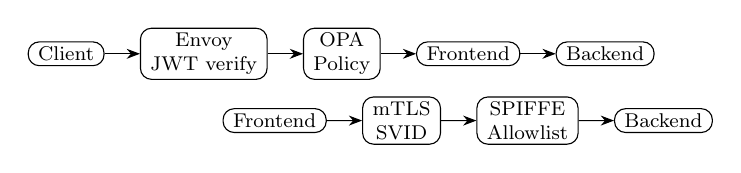
\begin{tikzpicture}[
    node distance=4mm and 5mm,
    every node/.style={draw, rounded corners, align=center, font=\footnotesize, inner xsep=4pt, inner ysep=2pt},
    >=Stealth,
    scale=0.9,
    transform shape
  ]
    \node (client) {Client};
    \node (envoy) [right=of client] {Envoy\\JWT verify};
    \node (opa) [right=of envoy] {OPA\\Policy};
    \node (frontend) [right=of opa] {Frontend};
    \node (backend) [right=of frontend] {Backend};
    \draw[->] (client) -- (envoy);
    \draw[->] (envoy) -- (opa);
    \draw[->] (opa) -- (frontend);
    \draw[->] (frontend) -- (backend);

    \node (frontend2) [below=of envoy, xshift=10mm] {Frontend};
    \node (mtls) [right=of frontend2] {mTLS\\SVID};
    \node (spiffe) [right=of mtls] {SPIFFE\\Allowlist};
    \node (backend2) [right=of spiffe] {Backend};
    \draw[->] (frontend2) -- (mtls);
    \draw[->] (mtls) -- (spiffe);
    \draw[->] (spiffe) -- (backend2);
  \end{tikzpicture}
  \caption{Request flow and enforcement layers.}
  \label{fig:arch}
\end{figure}

\section{Results}
\subsection{Scenario Outcomes}
All 20 test cases pass in the final validation run (see evidence/test-results.txt).
Table~\ref{tab:scenarios} summarizes the scenario outcomes.

\begin{table}[t]
\caption{Security scenario outcomes}
\label{tab:scenarios}
\centering
\footnotesize
\begin{tabularx}{\columnwidth}{l X l}
\toprule
Scenario & Threat and control & Result \\
\midrule
A & Lateral movement blocked by mTLS and SPIFFE allowlist & Blocked \\
B & Forged or tampered JWT rejected by JWKS verification & Blocked \\
C & Role + method + path enforced in OPA policy & Enforced \\
D & JWT claim-based authorization with Keycloak + OPA & Enforced \\
E & Device posture gate via policy condition & Enforced \\
\bottomrule
\end{tabularx}
\end{table}

\subsection{Scenario Details}
\textbf{A: Lateral movement (north-south and east-west).} The north-south baseline
confirms unauthenticated requests are denied, while a demo header allows access to
illustrate why header-only identity is weak. For east-west movement, a rogue pod
without a sidecar fails mTLS, and a pod with the wrong ServiceAccount is denied by the
SPIFFE allowlist. Direct pod IP access is also blocked. These tests validate workload
identity and service-to-service authorization as separate gates (Table~\ref{tab:scenario-a}).

\begin{table}[t]
\caption{Scenario A test matrix}
\label{tab:scenario-a}
\centering
\footnotesize
\begin{tabularx}{\columnwidth}{l X c c}
\toprule
Case & Request signals & Expect & Result \\
\midrule
A-NS-1 & GET \texttt{/api/admin}, no identity & 403 & 403 \\
A-NS-2 & GET \texttt{/api/admin}, header \texttt{role:admin} & 200 & 200 \\
A-EW-1 & Rogue pod without sidecar to backend & 403/000/503 & 403 \\
A-EW-2 & Wrong ServiceAccount to backend & 403 & 403 \\
A-EW-3 & Rogue pod to backend pod IP:8080 & 403/000/503 & 503 \\
\bottomrule
\end{tabularx}
\end{table}

\textbf{B: JWT forgery and tampering.} A forged JWT is rejected because no valid
principal is established at the mesh layer. A tampered payload with the original
signature fails cryptographic verification, returning a 401. A valid Keycloak-issued
JWT is accepted and passes to OPA for authorization (Table~\ref{tab:scenario-b}).

\begin{table}[t]
\caption{Scenario B test matrix}
\label{tab:scenario-b}
\centering
\footnotesize
\begin{tabularx}{\columnwidth}{l X c c}
\toprule
Case & Request signals & Expect & Result \\
\midrule
B-1 & Forged JWT to \texttt{/api/admin} & 403 & 403 \\
B-2 & Tampered real JWT to \texttt{/api/admin} & 401 & 401 \\
B-4 & Valid Keycloak JWT to \texttt{/api/admin} & 200 & 200 \\
\bottomrule
\end{tabularx}
\end{table}

\textbf{C: Context-based access control.} This scenario demonstrates that identity is
not enough: role, method, and path must be consistent. A user role can read
\texttt{/api/data} but is denied on \texttt{/api/admin} and all write operations, while
an admin role can write. This uses header-based roles as a deliberate baseline for
contrast with Scenario D (Table~\ref{tab:scenario-c}). In the final configuration,
JWT authentication is still enforced; the header-based rules illustrate why signed
claims are needed even when a request is authenticated.

\begin{table}[t]
\caption{Scenario C test matrix}
\label{tab:scenario-c}
\centering
\footnotesize
\begin{tabularx}{\columnwidth}{l X c c}
\toprule
Case & Request signals & Expect & Result \\
\midrule
C-1 & \texttt{role:user}, GET \texttt{/api/data} & 200 & 200 \\
C-2 & \texttt{role:user}, GET \texttt{/api/admin} & 403 & 403 \\
C-3 & \texttt{role:user}, POST \texttt{/api/write} & 403 & 403 \\
C-4 & \texttt{role:admin}, POST \texttt{/api/write} & 200 & 200 \\
\bottomrule
\end{tabularx}
\end{table}

\textbf{D: JWT claim authorization.} Authorization is driven by signed claims in the
JWT. An admin token can access admin endpoints, while a viewer token is limited to
read-only paths. This closes header spoofing and demonstrates a cryptographically
bound identity source of truth (Table~\ref{tab:scenario-d}).

\begin{table}[t]
\caption{Scenario D test matrix}
\label{tab:scenario-d}
\centering
\footnotesize
\begin{tabularx}{\columnwidth}{l X c c}
\toprule
Case & Request signals & Expect & Result \\
\midrule
D-1 & Admin JWT, GET \texttt{/api/admin} & 200 & 200 \\
D-2 & Viewer JWT, GET \texttt{/api/data} & 200 & 200 \\
D-3 & Viewer JWT, GET \texttt{/api/admin} & 403 & 403 \\
D-4 & Viewer JWT, POST \texttt{/api/write} & 403 & 403 \\
\bottomrule
\end{tabularx}
\end{table}

\textbf{E: Device posture gating.} Even with a valid admin JWT, access is denied when
the device posture signal indicates risk. The demo uses the \texttt{X-Device-Firewall}
header to model a health signal and illustrates how posture can be integrated into
policy decisions (Table~\ref{tab:scenario-e}).

\begin{table}[t]
\caption{Scenario E test matrix}
\label{tab:scenario-e}
\centering
\footnotesize
\begin{tabularx}{\columnwidth}{l X c c}
\toprule
Case & Request signals & Expect & Result \\
\midrule
E-1 & Admin JWT, \texttt{X-Device-Firewall: enabled} & 200 & 200 \\
E-2 & Admin JWT, \texttt{X-Device-Firewall: disabled} & 403 & 403 \\
\bottomrule
\end{tabularx}
\end{table}

\subsection{Operational Evidence}
OPA decision logs confirm allow and deny outcomes for each scenario, and the automated
``make test-all'' run provides a consolidated PASS summary. The evidence directory
includes detailed logs for JWT forgery, lateral movement attempts, and device posture
simulation.

\begin{figure}[H]
  \centering
  \fbox{\parbox[c][1.0in][c]{0.95\columnwidth}{\centering
  Placeholder: Kiali topology screenshot}}
  \caption{Service mesh topology (Kiali).}
  \label{fig:kiali}
\end{figure}

\subsection{Performance}
Performance testing uses Fortio with 200 requests and a single connection. Results are
shown in Table~\ref{tab:perf}.

Table~\ref{tab:policy-cost} provides a supplemental view of per-scenario timing for
representative allowed and blocked requests. Blocked cases measure policy decision
cost only (the request is denied before application handling). Allowed cases include
end-to-end handling, so the two categories should be interpreted separately.

\begin{table}[t]
\caption{Performance impact (200 requests, single connection)}
\label{tab:perf}
\centering
\footnotesize
\begin{tabular}{lccc}
\toprule
Metric & Baseline & ZTA & Delta \\
\midrule
Avg latency & 5.33 ms & 6.86 ms & +1.53 ms (+28.6\%) \\
QPS & 187.5 & 145.7 & -41.8 (-22.3\%) \\
p99 latency & 8.5 ms & 10.5 ms & +2.0 ms (+23.5\%) \\
\bottomrule
\end{tabular}
\end{table}

\begin{table}[t]
\caption{Per-scenario latency: allow = end-to-end, block = policy gate only (Fortio, 200 requests)}
\label{tab:policy-cost}
\centering
\footnotesize
\begin{tabularx}{\columnwidth}{l l X r r r}
\toprule
Case & Type & Request signal & Avg (ms) & p99 (ms) & Code \\
\midrule
A1 & Allow & Admin JWT, GET \texttt{/api/admin} & 5.94 & 7.89 & 200 \\
A2 & Allow & Viewer JWT, GET \texttt{/api/data} & 6.63 & 8.80 & 200 \\
A3 & Allow & \texttt{role:user}, GET \texttt{/api/data} & 6.58 & 9.00 & 200 \\
A4 & Allow & Admin JWT + \texttt{X-Device-Firewall: enabled} & 6.22 & 7.94 & 200 \\
B1 & Block & No identity, GET \texttt{/api/admin} & 2.02 & 4.00 & 403 \\
B2 & Block & Forged JWT, GET \texttt{/api/admin} & 2.36 & 5.00 & 403 \\
B3 & Block & Tampered JWT, GET \texttt{/api/admin} & 2.00 & 4.00 & 401 \\
B4 & Block & Admin JWT + \texttt{X-Device-Firewall: disabled} & 2.91 & 5.50 & 403 \\
\bottomrule
\end{tabularx}
\end{table}

\begin{figure}[H]
  \centering
  \fbox{\parbox[c][1.0in][c]{0.95\columnwidth}{\centering
  Placeholder: Grafana latency dashboard screenshot}}
  \caption{Latency and throughput metrics (Grafana).}
  \label{fig:grafana}
\end{figure}

\section{Discussion}
\subsection{Security Value vs Traditional Controls}
The implementation demonstrates that per-request authorization at the infrastructure
layer can block attack paths that traditional perimeter controls miss. Even with valid
credentials, requests are denied when policy context is violated, and internal lateral
movement is blocked by workload identity checks.

\subsection{VPN vs ZTA}
WireGuard provides low-overhead transport security but does not enforce request-level
authorization or workload identity. ZTA adds these controls with a measurable overhead,
so the most practical deployment is layered: VPN for secure entry and ZTA for service
policy enforcement.

\section{Limitations}
Device posture is simulated through a client-provided header, and the OPA ext-authz
channel is not mTLS-encrypted due to sidecar dependency constraints. Header-based role
rules remain in place to demonstrate weaker access controls (Scenario C) alongside the
stronger JWT claim path (Scenario D). The scenario set is representative but not
exhaustive, and ZTA does not eliminate risks from human error, misconfiguration, or
novel low-level exploits. The environment is local and does not represent production-
scale latency or throughput.

\section{Experience and Reflection}
\subsection{Unexpected Outcomes}
I expected the implementation to be harder, but the core ZTA flow was manageable once
the stack was aligned. The most surprising result was performance overhead: the
latency increase and QPS drop were higher than I anticipated, even in a small test.

\subsection{Implementation Challenges}
The initial setup and integration of Istio, OPA, and Keycloak was the most time-
consuming part. JWT verification flow and automated end-to-end tests required careful
ordering and debugging. I also spent time looking for missing scenarios and thinking
about bypasses not captured by the default test set.

\subsection{Limits of ZTA and Current Practice}
This project reinforced that ZTA is a strong practical approach but not perfect. It
does not eliminate risks from human error, system misconfiguration, or novel low-level
exploits, and it only blocks the scenarios it explicitly models. AI-assisted work
helped accelerate policy iteration, but it did not remove the need for manual
validation, and it reminded me that attackers can also use AI to discover new paths.
ZTA feels like the best available option today, not a final solution.

\subsection{Lessons Learned and Future Work}
I learned that layered controls matter more than any single tool, and that the
security-performance trade-off is real. As hardware improves, some overhead will be
easier to absorb, but the dilemma remains. If I extend this work, I want to design a
more efficient policy path and push enforcement closer to lower-level boundaries so
that isolation holds even against unexpected paths.

\section{Conclusion}
The sandbox validates that open-source tools can implement a realistic Zero Trust
Architecture aligned with NIST SP 800-207. The system blocks five representative
attack scenarios and provides clear audit evidence for each decision. The measured
performance cost is acceptable for a security-focused environment, and the design
illustrates how identity, context, and workload trust can replace implicit network
trust.

\begin{thebibliography}{1}
\bibitem{nist}
NIST, ``Zero Trust Architecture,'' SP 800-207, 2020.\newline
\url{https://csrc.nist.gov/publications/detail/sp/800-207/final}

\bibitem{beyondcorp}
Google, ``BeyondCorp: A New Approach to Enterprise Security,'' 2014.\newline
\url{https://research.google/pubs/pub43231/}

\bibitem{wireguard}
J. A. Donenfeld, ``WireGuard: Next Generation Kernel Network Tunnel,'' 2017.\newline
\url{https://www.wireguard.com/papers/wireguard.pdf}
\end{thebibliography}

\end{document}
